\documentclass[12pt]{article}

% = Подключение пакетов =
%  - Поддержка русских букв -
\usepackage[T1,T2A]{fontenc}
\usepackage[utf8]{inputenc}
\usepackage[english,russian]{babel}
%  - Размеры полей -
\usepackage[right=1.5cm,top=2cm,left=3cm,bottom=2cm]{geometry}
%  - Отступ в начале первого абзаца -
\usepackage{indentfirst}
%  - Титульный лист с содержанием -
\usepackage{practice}
%  - Гиперссылки (url, \ref-ссылки, \cite-ссылки)
\usepackage{hyperref}
%  - Отображение математических формул
\usepackage{amsthm,amssymb,amsmath}

% = Общие настройки =
%  - Полуторный межстрочный интервал -
\linespread{1.5}
%  - Разрешить разреженные строки и запретить перенос -
\sloppy
\hyphenpenalty=10000
\exhyphenpenalty=10000


% = (!!!) Здесь впишите свои данные =
%  - Название работы -
\prTitle{Поиск быстрых алгоритмов умножения матриц}
%  - Как вас зовут, В РОДИТЕЛЬНОМ ПАДЕЖЕ -
\prAuthor{Баканова Артёма Михайловича}
%  - Степень, должность и Фамилия И.О. научного руководителя -
\prSupervisorTitle{д.ф.-м.н.,~проф.}
\prSupervisorName{Алексеев~В.\,Б.}
%  - Степень (если есть), должность и Фамилия И.О. руководителя практики от факультета -
\prBossTitle{д.ф.-м.н.,~проф.}
\prBossName{Алексеев~В.\,Б.}
%  - Если показывается неправильный год, то раскомментируйте и напишите правильный -
% \prYear{2019}

\begin{document}
    \prPutTitleContents


    \section{Введение}

    Умножение матриц является одной из фундаментальных операций в линейной алгебре и широко используется в различных
    приложениях, таких как машинное обучение, компьютерное зрение и обработка сигналов.
    Однако, найти оптимальный алгоритм умножения матриц является сложной задачей.

    Традиционно сложность алгоритмов умножения матриц оценивается в количестве операций умножения чисел.
    Это связано с тем, что последняя является наиболее ресурсозатратной.
    Таким образом, оптимальный алгоритм должен выигрывать у остальных по числу умножений.
    Так, стандартный алгоритм умножения матрицы $ m \times n $ на матрицу $ n \times p $
    \begin{equation}
        z_{ij} = \sum_{k=1}^{n} x_{ik} y_{kj},
        \quad i = \overline{1,m}, \: j = \overline{1,p}\label{eq:1}
    \end{equation}
    требует $ n^3 $ операций умножения, то есть имеет асимптотическую сложность $ \mathcal{O}(n^3) $.

    Крайне важным шагом в поиске быстрых алгоритмов стала работа Штрассена~\cite{strassen}.
    В ней он приводит алгоритм умножения двух квадратных матриц порядка $ n $ с асимптотической сложностью
    $ \mathcal{O}(n^{\log_2 7}) $.
    Алгоритм Штрассена основан на том, что для умножения квадратных матриц порядка $ 2 $ требуется лишь $ 7 $ операций
    умножения.


    \section{Постановка задачи}

    Козловым Александром была написана программа, вычисляющая решение системы для переменных (0), (2), (3), (4), (5),
    (6) с невязкой порядка $ 10^{-6} $.
    Передо мной ставилась задача попытаться расширить данные решения для переменных (7) и (8) на множестве комплексных
    чисел.


    \section{Полученные результаты}

    \subsection{Краткое напоминание предыдущих итогов работы}

    Исходя из системы

    \begin{equation}
        \sum_{d=1}^{q} \alpha_{ij} \beta_{kl} \gamma_{rs} =
        \begin{cases}
            1,\text{ если } j = k, l = r, s = i;\\
            0, \text{ иначе.}
        \end{cases}\label{eq:2}
    \end{equation}

    и используя ряд предположений, была получена новая система.
    Левая часть уравнения системы для тройки $(m, p, q)$ имеет вид

    \begin{gather*}
        2\cdot (x_{m} y_{p} z_{q}+x_{p} y_{q} z_{m}+x_{q} y_{m} z_{p}) +\\
        +2 \cdot (\varphi_2 (x_m) \varphi_2 (y_p) \varphi_2 (z_q)+ \varphi_2 (x_p) \varphi_2 (y_q) \varphi_2 (z_m)+ \varphi_2 (x_q) \varphi_2 (y_m) \varphi_2 (z_p))+\\
    \end{gather*}
    \begin{equation}
        +\sum_{d=3}^{6} (\varphi_d (a_m) \varphi_d (b_p) \varphi_d (c_q)+ \varphi_d (a_p) \varphi_d (b_q) \varphi_d (c_m) + \varphi_d (a_q) \varphi_d (b_m) \varphi_d (c_p)).\label{eq:3}
    \end{equation}

    а правая часть определяется, как

    \begin{equation}
        \sum_{i,j,k,l,r,s=0}^2 t_{ij}^{(m)} t_{kl}^{(p)} t_{rs}^{(q)} f_{ij,kl,rs}.\label{eq:4}
    \end{equation}

    \subsection{Отсеивание решений}

    Поскольку программа Александра умеет генерировать практически бесконечное число потенциальных решений, необходимо
    эффективно отбирать их.

    Если среди исходных $ 125 $ уравнений оставить только те, которые включают в себя переменные групп (7) и (8), то их
    останется ровно 65.
    При этом после подстановки решения $ 49 $ из них оказываются линейными.
    Это даёт нам возможность не искать сразу решение в общем случае сложными алгоритмами, а попытаться проанализировать
    линейную систему.
    Если система разрешима, то отбираем решение с минимальной невязкой и по её значению решаем, продолжать ли поиски в
    поле комплексных чисел.

    Было сгенерировано и проанализировано $ 1000 $ решений.
    Для каждого вычислялась минимальная невязка на линейной подсистеме.
    Результаты приведены на изображении ниже.

    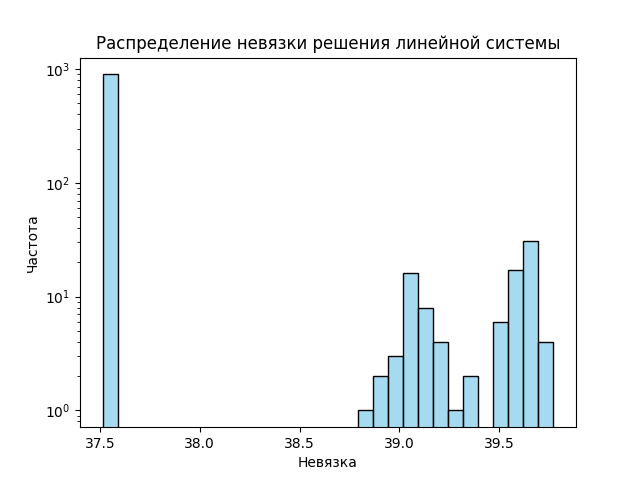
\includegraphics{linear.png}

    Таким образом, нет смысла пытаться дополнять данные решения значениями для переменных (7) и (8).
    Все они дают большую невязку уже на линейной подсистеме.

    \subsection{Пересчёт невязки}

    Стало интересно проверить, действительно ли решения Александра получаются с невязкой порядка $ 10^{-6} $.
    Были отобраны 60 уравнений, которые содержат только переменные групп $ (0)-(6) $.
    Для тех же 1000 решений невязка считалась, как евклидова норма вектора разности левой и правой частей уравнений.
    Полученные результаты отображены ниже.

    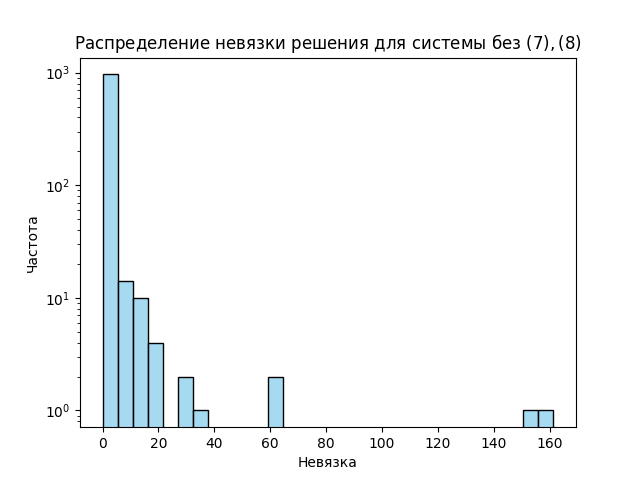
\includegraphics{prev.png}

    Соответственно, минимальное значение невязки, которое было получено, имеет порядок $10^{-3}$.
    Также встречаются решения с аномально большой невязкой.

    \subsection{Сравнение систем}

    После такого расхождения в невязке было принято решение программно сравнить коэффициенты уравнений системы
    Козлова и моей системы.
    Для каждой тройки $ (m, p, q) $ с точностью до эквивалентных перестановок коэффициенты уравнения совпали.
    Различия заключаются лишь в том, что в моей системе присутствует уравнение для тройки $ (1, 1, 1) $, которое имеет
    вид


    \begin{equation}
        a_{1}b_{1}c_{1} + x_{1}y_{1}z_{1} = 2\label{eq:5}
    \end{equation}

    На значение невязки оно принципиально не влияет.


    \section{План дальнейших работ}

    Разработать новые подходы к исследованию возможности существования решения с малой невязкой для рассматриваемой задачи, разработать для них алгоритмы и программы и провести эксперименты.

    \addcontentsline{toc}{section}{Список литературы}%
    \begin{thebibliography}{99}
        \bibitem{strassen} Strassen~V.\, Gaussian elimination is not optimal~// Numer. Math. 1969, том~13. С.~354--356.
    \end{thebibliography}
\end{document}
